\documentclass[12pt]{IEEEtran}
\usepackage{tikz}
\usepackage{../../../template}
\title{Conductivity in 3 Dimensions}
\author{Daniel Chua}
\begin{document}
\maketitle

\begin{abstract}
This paper investigates the behaviour of electrical conduction in different media in different dimensions, which are approximated by 3D geometry. Theoretical models are developed to solve for electrical resistivity. Arrays of voltmeter and current source (Wenner and Schlumberger) are used to test these equations, with varying levels of success. The models perform as expected only when edge effects are minimized, for example when a large piece of material is used.
\end{abstract}

\section{Introduction}

Electric fields are widely used in many fields in Physics. For example, they are used in Hall sensors, which make use of the Hall effect to detect magnetic fields. There are also applications in understanding superconductors, where there is ongoing experimentation on the behaviour of electric fields due to the lack of a voltage gradient in the material. In light of the above, further development into the theory of how electric fields propagate in different dimensions can help make sense of measurement results in these different applications.

In this experiment, the behaviour of electric fields is investigated in the 1D, 2D and 3D cases. In deriving relations, the following formulae from basic electrodynamics would be useful. We can relate electric field with current density by

\begin{equation} \label{current}
    \vec E = \rho \vec J
\end{equation}

We can also relate it with voltage gradient.

\begin{equation} \label{voltage}
    \vec E = -\nabla V
\end{equation}

Finally, current density can be used to find current by integrating

\begin{equation} \label{density}
    I = \int_A j(\vec r) dA
\end{equation}

This can usually be simplified to $I = JA$ assuming current density is constant. \\

For a 1D conductor, current density is a function of the scalar $x$ only. It has to be a constant due to conservation of charge. Velocity is a function of 1 variable, and its gradient can be written as a scalar. Then equations \ref{current}, \ref{voltage}, \ref{density} give

\begin{equation} \label{1D}
    \rho = \frac{VA}{bI}
\end{equation}

where $A$ is the cross-sectional area of the sheet. \\
For a 2D conductor, consider an infinitely large sheet. Current density in \ref{density} is integrated over an area of $2\pi ad$.

\begin{equation}\label{2D}
    \rho = \frac{2\pi adV}{bI}
\end{equation}

We similarly get to the 3D case. If we measure along a surface, the current density at a distance $a$ from the source becomes $I$ divided by the hemisphere with said radius. Derivation proceeds similarly. In addition, we use a 2 layer model in the experiment, where the resistivity $\rho(0 > z > l) = \rho_a$ on the surface layer is different from that of the deeper layer $\rho(z < l) = \rho_l$ at distance $l$ underground. A Wenner array is used, with $a=b$, simplifying the equation to

\begin{equation}
    \rho = \frac{2\pi aV}{I}
\end{equation}

Finally, a recurring topic in this report is edge effects. In ideal cases, current moves unobstructed, and the boundaries of the conductor is thought to be infinitely far away. In reality, this does not hold. Current is reflected as it reaches the boundary of the conductor, and this can challenge assumptions. On a 2D surface, one would expect current from a source to spread evenly outwards, where half the current goes to the left, and the other half to the right. For a source places near the left boundary, a greater portion of current would travel rightwards. A key assumption in the derivation of equations above is that current spreads evenly, given the degrees of freedom it enjoys depending on the dimension. Its failure affects the validity of these equations.

\section{Experimental Techniques}

\subsection{Methods}

We use Wenner and Schlumberger arrays, as depicted \ref{array}. In both cases, 4 probes are arranged linearly, with the current probes on the outside and the voltage probes on the inside. The current probes supply a constant current, and the voltage probes deliver voltage readings. In a Schlumberger array, $b << a$, while in a Wenner array, $b = a$. The Schlumberger array is used in 1D and 2D experiments, while the Wenner array is used in the 3D case. In practice, $b << a$ is realised as $\frac{a}{b} \geq 10$.

\begin{figure} \label{array}
    \begin{center}
    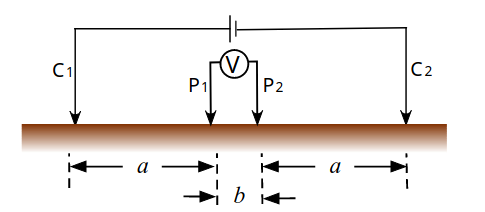
\includegraphics[scale=0.5]{array.png}
    \caption{Setup of Wenner and Schlumberger Arrays~\cite{manual}}
    \end{center}
\end{figure}
    
For small $a$, the recorded $\rho$ should be close to $\rho_a$. To find both $\rho_a$ and $\rho_l$, curve matching can be used. In cases where $\rho_a << \rho_l$, less current penetrates the second layer, so more passes through the voltage probes, giving a higher voltage reading. This effect depends on $a$, and one can plot $\rho$ against $a$ to determine both resistivities. The curve of $\frac{\rho_a}{\rho_l}$ against $\frac{a}{d}$ is completely determined by the reflection coefficient

\begin{equation}
    \kappa = \frac{\rho_l-\rho_a}{\rho_l+\rho_a}
\end{equation}

which is approximated as 1, since $\rho_{\text{air}} >> \rho_{\text{graphite}}$. The curve is generated by \verb|wenner_array_curve_finite_slab.py|, which can be found in \ref{code}.

\subsection{Procedures}

Aluminimum foil, a graphite slab, 2 voltage probes, and 2 current probes are used. Aluminium foil and the slab are used as conductors respectively. Conductivity of both are assumed to be relatively constant, and literature values are readily available. One side of the foil is oxidized, which may affect conductivity. For consistency, the oxide layer is \textit{not} used. \\
For the 1D case, a thin strip of aluminimum foil is used, and the probes are placed along the axis, with $b << a$. The strip is produced carefully with scissors, but it is difficult to create an ideal rectangular shape. Width varies along the length, but great care is taken in ensuring that the width is constant in the area between the voltmeter probes. \\
For the 2D case, a sheet of aluminium foil is used, and the probes are placed either along the longer edge or the diagonal, with $b << a$. As $b$ grows, it is unavoidable that the current probes get closer to the boundaries, and edge effects become important. \\
For the 3D case, the graphite slab is used, and the probes are placed in the same arrangements as in the 2D case, but with $b = a$ instead. \\
For the Schlumberger arrays, $b$ is fixed while $a$ varies. For the Wenner arrays, $a$ varies.

\section{Results and Discussion} 

\subsection{1D case}

$a = 14.5 \pm 0.1\unit{cm}, b = 1.0 \pm 0.1\unit{cm}, h = 0.016 \unit{mm}, w = 1.3 \pm 0.1\unit{cm}, V = 1.89 \pm 0.005 \unit{mV}, I = 1.0 \pm 0.025 \unit{A}$, where $w$ and $h$ denote width and height respectively. From \ref{1D}, resistivity is predicted to be
$$\rho = (3.9 \pm 0.5) \times 10^{-8} \unit{\Omega.m}$$

This agrees with the literature value~\cite{al} of $2.82 \times 10^{-8} \unit{\Omega.m}$.

The major source of error comes from sheet geometry and measurements. As explained, width varies along the length of the strip. Validity of the equation depends on an accurate estimate of current density along the voltage gradient, which depends on width, thus greater care is taken on the sheet segment lying between the probes to reduce error. Nevertheless, measurement uncertainties are relatively large. They have a constant value determined by the smallest spacings on the ruler, and percentage significance grows with a small width.

\subsection{2D case}

\begin{figure}[h]
\begin{center}\label{2ddata}
\scalebox{0.7}{
\begin{tabular}{|c|c|c|c|c|}
    \hline
    a (cm) & b (cm) & I (A) & V (mV) & $\rho (\unit{\Omega.m})$ \\
    \hline\hline
    $5.0 \pm 0.1$ & $0.5 \pm 0.1$ & $1 \pm 0.025$ & $0.083 \pm 0.0005$ & $8 \pm 2 \times 10^{-8}$ \\
    \hline
    $12.0 \pm 0.1$ & $0.5 \pm 0.1$ & $1 \pm 0.025$ & $0.043 \pm 0.0005$ & $1.0 \pm 0.2 \times 10^{-7}$ \\
    \hline
    $13.0 \pm 0.1$ & $0.5 \pm 0.1$ & $1 \pm 0.025$ & $0.042 \pm 0.0005$ & $1.1 \pm 0.2 \times 10^{-7}$ \\
    \hline
    $16.0 \pm 0.1$ & $0.5 \pm 0.1$ & $1 \pm 0.025$ & $0.035 \pm 0.0005$ & $1.1 \pm 0.2 \times 10^{-7}$ \\
    \hline
    $16.0 \pm 0.1$ & $0.5 \pm 0.1$ & $1 \pm 0.025$ & $0.035 \pm 0.0005$ & $1.1 \pm 0.2 \times 10^{-7}$ \\
    \hline
    $18.0 \pm 0.1$ & $0.5 \pm 0.1$ & $1 \pm 0.025$ & $0.040 \pm 0.0005$ & $1.5 \pm 0.3 \times 10^{-7}$ \\
    \hline
    $23.0 \pm 0.1$ & $0.5 \pm 0.1$ & $1 \pm 0.025$ & $0.039 \pm 0.0005$ & $1.1 \pm 0.4 \times 10^{-7}$ \\
    \hline
\end{tabular}}
\caption{2D Data}
\end{center}
\end{figure}

Different trials with varying $a,b,I,V$ are taken. Resistivity is calculated from \ref{2D}. From the data, it can be seen that the values for $\rho$ are greater than in the first experiment. A possible explanation is that if the current source is too close to the edges of the conductor, current density at the voltmeter is greater than expected, since current is distributed over an arc instead of the entire circle; see \ref{partial}. From equation \ref{current}, if we use the actual greater value of $\vec J$, we should obtain a smaller $\rho$, which agrees with our findings. Also, the greater $a$ is, the more significant this effect is, which agrees with the general trend of the calculated $\rho$ increasing with $a$. Further experimentation, if possible, could determine the relationship between the calculated and actual values of resistivity. \\
Edge effects lead to $\rho$ values being multiples larger than actual values. This outweighs all potential sources of error.

\begin{figure}[h]
\begin{center}
\begin{tikzpicture}\label{partial}
    % Rectangle
    \draw (0,0) rectangle (8,4.5);

    % Clip to only show the bottom right part of the circle and arrows
    \begin{scope}
        \clip (0,0) rectangle (8,4.5);
        
        % Circle centered at the top left corner of the rectangle
        \draw (1,4) circle (2);

        % Arrows pointing out from the clipped circle
        \foreach \angle in {30, 60, ..., 360}
            \draw[->] (1,4) -- ++(\angle:2);
    \end{scope}
\end{tikzpicture}
\end{center}
\caption{Current spreads along an arc instead of circumference}
\end{figure}

\subsection{3D case}

Theoretically, the same difficulties in the 2D case would be present here. However, since the depth $l$ of the surface layer is very thin, around 5 cm, this overshadows edge effects which become significant at around $a = 10\unit{cm}$.

\begin{figure}[h]
\begin{center}\label{3ddata}
    \scalebox{0.7}{
    \begin{tabular}{|c|c|c|c|}
        \hline
        a (cm) & I (A) & V (mV) & $\rho_a (\Omega m)$ \\
        \hline\hline
        $1.5 \pm 0.1$ & $1 \pm 0.025$ & $0.865 \pm 0.0005$ & $9.1 \pm 0.6 \times 10^{-5}$ \\
        \hline
        $1.7 \pm 0.1$ & $1 \pm 0.025$ & $0.908 \pm 0.0005$ & $9.7 \pm 0.6 \times 10^{-5}$ \\
        \hline
        $2.0 \pm 0.1$ & $1 \pm 0.025$ & $0.825 \pm 0.0005$ & $1.04 \pm 0.06 \times 10^{-4}$ \\
        \hline
        $2.2 \pm 0.1$ & $1 \pm 0.025$ & $0.730 \pm 0.0005$ & $1.01 \pm 0.05 \times 10^{-4}$ \\
        \hline
        $2.5 \pm 0.1$ & $1 \pm 0.025$ & $0.647 \pm 0.0005$ & $1.02 \pm 0.05 \times 10^{-4}$ \\
        \hline
        $2.7 \pm 0.1$ & $1 \pm 0.025$ & $0.598 \pm 0.0005$ & $1.01 \pm 0.05 \times 10^{-4}$ \\
        \hline
        $3.0 \pm 0.1$ & $1 \pm 0.025$ & $0.566 \pm 0.0005$ & $1.07 \pm 0.05 \times 10^{-4}$ \\
        \hline
        $4.0 \pm 0.1$ & $1 \pm 0.025$ & $0.482 \pm 0.0005$ & $1.21 \pm 0.04 \times 10^{-4}$ \\
        \hline
        $5.0 \pm 0.1$ & $0.95 \pm 0.025$ & $0.452 \pm 0.0005$ & $1.49 \pm 0.05 \times 10^{-4}$ \\
        \hline
        $10.0 \pm 0.1$ & $0.95 \pm 0.025$ & $0.444 \pm 0.0005$ & $2.94 \pm 0.09 \times 10^{-4}$ \\
        \hline
        $15.0 \pm 0.1$ & $0.95 \pm 0.025$ & $0.519 \pm 0.0005$ & $5.2 \pm 0.1 \times 10^{-4}$ \\
        \hline
        $20.0 \pm 0.1$ & $0.95 \pm 0.025$ & $0.619 \pm 0.0005$ & $8.2 \pm 0.2 \times 10^{-4}$ \\
        \hline
        $25.0 \pm 0.1$ & $0.95 \pm 0.025$ & $0.730 \pm 0.0005$ & $1.21 \pm 0.03 \times 10^{-3}$ \\
        \hline
        $30.0 \pm 0.1$ & $0.95 \pm 0.025$ & $0.881 \pm 0.0005$ & $1.75 \pm 0.05 \times 10^{-3}$ \\
        \hline
\end{tabular}}
    \caption{3D Data}
\end{center}
\end{figure}

Data from different Wenner arrangements can be found in table \ref{3ddata}. Since the graphite slabs have finite thickness, we take $\rho_a = \rho_{\text{graphite}}$ and $\rho_l = \rho_{\text{air}}$. The theory behind curve matching will not be covered in this paper; see~\cite{curve}. The model (Figure \ref{odr}) yields a thickness of $5.33 \pm 0.08 \unit{cm}$ for the graphite slab with a resistivity of $9.4 \pm 0.2 \times 10^{-5} \unit{\Omega.m}$, which agrees with a literature value~\cite{res} of $6 \times 10^{-5} \unit{\Omega.m}$. See \verb|odr_fit_extended.py| in \ref{code} for the implementation, where orthogonal distance regression is used for curve fitting. \\

Sources of error mostly come from measurements. For greater values of $a$, they can be bounded.

\begin{figure}\label{odr}
    \begin{center}
    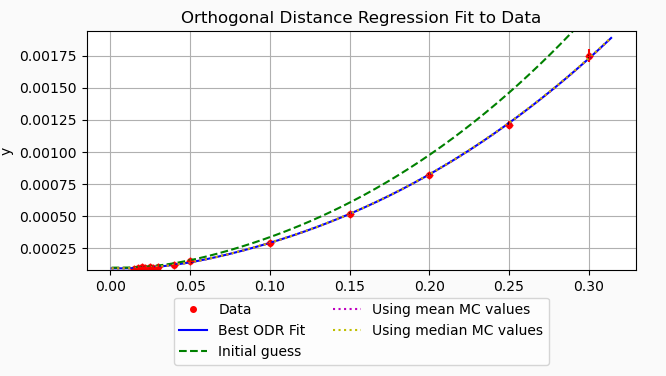
\includegraphics[scale=0.5]{odrfit.png}
    \end{center}
\end{figure}

\section{Conclusion}

This paper investigates the behaviour of conduction in various dimensions. Theoretical models are built, which predict resistivity given sufficient parameters. These equations are tested by solving for known resistivities of aluminium and graphite. The models for 1D and 3D conduction are validated, and extra care is needed for the model for 2D conduction, where further research is required to investigate geometry-dependent behaviour. In general, as long as conduction occurs far away from the edges, these results support the intuition that current spreads symmetrically through space, since it is the underlying assumption in the derivation of the equations.

\appendix

\section{Code} \label{code}

The code used in this report, including \verb|wenner_array_curve_finite_slab.py|, the \verb|csv| file it generates (\verb|wenner_array_finite_slab.csv|), and \verb|odr_fit_extended.py| can be found at \url{https://github.com/latexsupremecist/EngSci/tree/main/PHY327/C3D}.

\bibliography{refs.bib}{}
\bibliographystyle{IEEEtran}
\end{document}
